\subsubsection{Iteration 3: Evaluation}

This iteration focus on refining the PID Controller and evaluation on the agent.

\paragraph{Design}

To refine the PID Controller, the joystick update pace was adjusted into 20 frame one update. And I also adjusted the PID parameters showed in \cref{table:pid_params}

\begin{table}[h]
\centering
\caption{PID Controller Parameters} \label{table:pid_params}
\begin{tabular}{lccccc}
\hline
\textbf{Controller} & \textbf{Axis} & $K_p$ & $K_i$ & $K_d$ & Max Output \\
\hline
Position (Outer Loop) & X & 2.0 & 0.10 & 1.5 & 10 \\
Position (Outer Loop) & Y & 3.0 & 0.12 & 1.5 & 15 \\
Position (Outer Loop) & Z & 2.0 & 0.10 & 1.5 & 10 \\
\hline
Velocity (Inner Loop) & X & 1.0 & 0.05 & 0.3 & 8 \\
Velocity (Inner Loop) & Y & 1.5 & 0.10 & 0.5 & 12 \\
Velocity (Inner Loop) & Z & 1.0 & 0.05 & 0.3 & 8 \\
\hline
Yaw Control & Yaw & 3.0 & 0.00 & 1.0 & 5 \\
\hline
\end{tabular}
\end{table}

\paragraph{Enact}

In the hovering task, the newly refined PID controller can provide satisfied result. Ilustrated in \cref{fig:rl_hover}, The two agents, PID(orange) and RL(blue) were set to hover on a stable 5m height. The data was collected in 60s. From the data, the refined PID controller can finish the hovering stably while RL agent was more moving around the line.

\begin{figure}[H]
    \caption{Hovering task result, throttle value on the top, drone's height in the bottom}\label{fig:rl_hover}
    \centering
    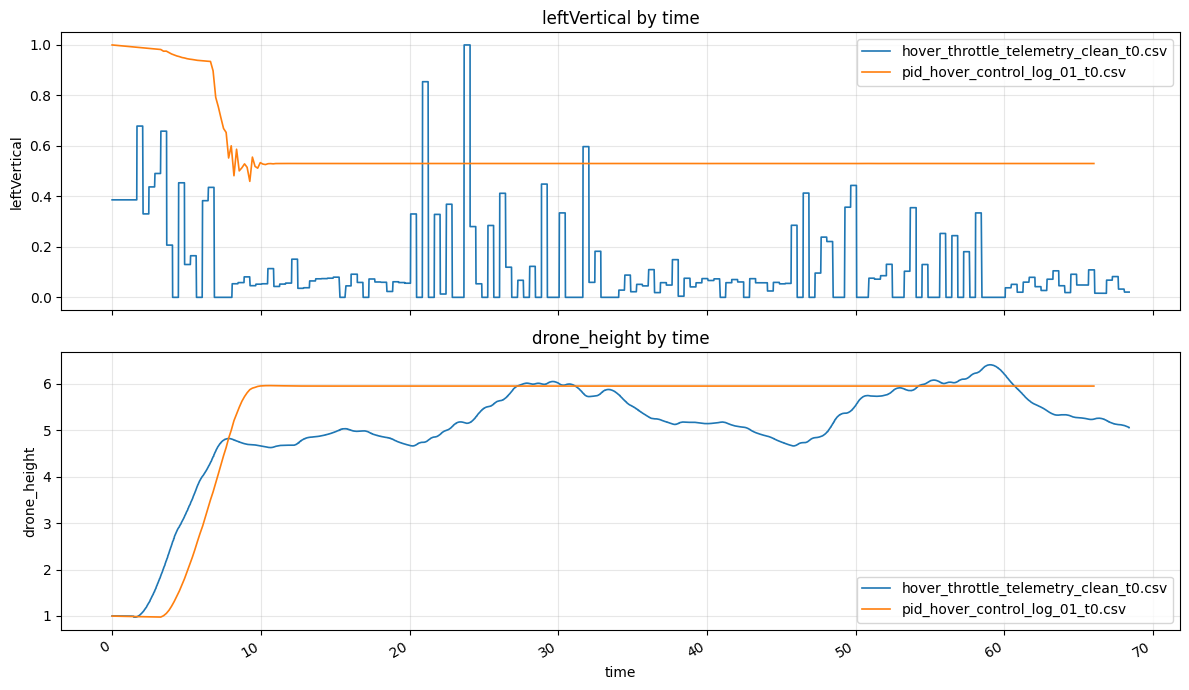
\includegraphics[width=0.8\linewidth]{img/result_hovering.png}
\end{figure}